%%\documentclass[a4paper, 12pt]{scrreprt}

\documentclass[a4paper, 12pt]{scrartcl}
%usepackage[german]{babel}

%\usepackage{amsmath}
%usepackage{color}
\usepackage[utf8]{inputenc}
\usepackage[T1]{fontenc}
\usepackage{wrapfig}
\usepackage{lipsum}% Dummy-Text

%%%%%%%%%%%%bis hierhin alle nötigen userpackage

\usepackage[utf8]{inputenc}
\usepackage{amsmath}
\usepackage{amsfonts}
\usepackage{amssymb}
\usepackage{graphicx}
%\usepackage{wrapfig}
\usepackage[ngerman]{babel}
\usepackage[left=25mm,top=25mm,right=25mm,bottom=25mm]{geometry}
%\usepackage{floatrow}
\setlength{\parindent}{0em}
\usepackage[font=footnotesize,labelfont=bf]{caption}
\numberwithin{figure}{section}
\numberwithin{table}{section}
\usepackage{subcaption}
\usepackage{float}
\usepackage{url}
\usepackage{fancyhdr}
\usepackage{array}
\usepackage{geometry}
%\usepackage[nottoc,numbib]{tocbibind}
\usepackage[pdfpagelabels=true]{hyperref}
\usepackage[font=footnotesize,labelfont=bf]{caption}
\usepackage[T1]{fontenc}
\usepackage {palatino}
%\usepackage[numbers,super]{natbib}
%\usepackage{textcomp}
\usepackage[version=4]{mhchem}

%\begin{document}

\newcolumntype{L}[1]{>{\raggedright\arraybackslash}p{#1}} % linksbündig mit Breitenangabe
\newcolumntype{C}[1]{>{\centering\arraybackslash}p{#1}} % zentriert mit Breitenangabe
\newcolumntype{R}[1]{>{\raggedleft\arraybackslash}p{#1}} % rechtsbündig mit Breitenangabe

\section{Zusammenfassung}

Die erhaltenen Werte stimmen gut mit den Literaturwerten überein.\ref{Literatur}. 
Die mittels der CCSD-Methode gewonnenen Werte nähern sich besser an den Gleichgewichtsabstand der Literatur an. Die Dissoziationsenergien, welche durch die B3LYP-Methode erhalten werden, entsprechen eher den Literaturwerten, jedoch decken sich die berechneten Werte alle wesentlich schlechter mit der Literatur als es bei dem Gleichgewichtsabstand der Fall ist. 


\section{Auswertung}


Die mittels Gaussian erhaltenen Gleichgewichtsabstände wurden in Tabelle \ref{Tab.1} zusammengetragen. Dabei handelt es sich um den Atomabstand R, welcher bei den jeweiligen minimalsten Energiewerten einer Datenreihe zu finden ist. Die Dissoziationensenergie wurden erhalten, indem der größte Energiewert der Asymptote vom kleinsten Energiewert der Kurve subtrahiert worden ist.

 \begin{table}[H]
 \centering
 \caption{Berechnete Gleichgewichtsabstände und Dissoziationsenergien aus den mittels GAUSSIAN erhaltenen Werten}
 \begin{tabular}{L{0.1\textwidth}L{0.20\textwidth}C{0.4\textwidth}C{0.30\textwidth}}

 
  Molekül  & Methode& Gleichgewichtsabstand R in Ängstrom &  Dissoziationsenergie in Einheit?? \\
  CO  &B3LYP &1.17 &  0.48 \\
  CO  & CCSD (SCF)&1.11 & 0.49\\
  CO  & CCSD (MP2)&1.15 & 0.59\\
  CO  & CCSD (MP3)&1.13 & 0.16\\
  HCl  &B3LYP& 1.33 &  0.19\\
  HCl  & CCSD (SCF)&1.27  & 0.34\\
  HCl  & CCSD (MP2)&1.28  & 0.19\\
  HCl  & CCSD (MP3)&1.28  & 0.16\\
  
 \end{tabular}
 \label{Tab.1}
 \end{table}
 
 
\begin{figure}[ht]
	\centering	
	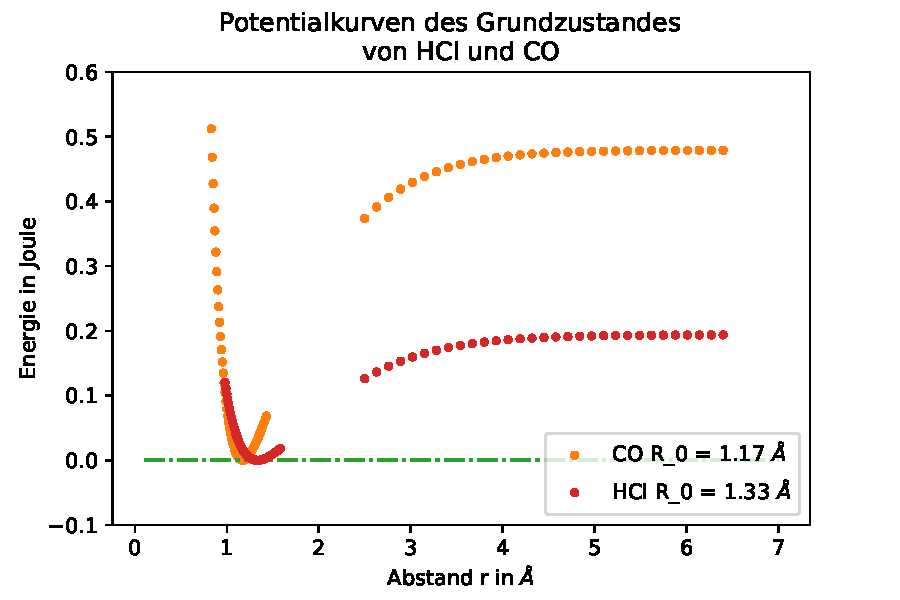
\includegraphics[width=\columnwidth]{Bilder/b3lypzusammen}
	\caption{Was ist eine Caption}
	\label{b3lypzusammen}
\end{figure}


Wie in Abbildung \ref{b3lypzusammen} zu sehen beschreiben die mit B3LYP errechneten Werte den Verlauf eines Morsepotentials. Es sei hier erwähnt, dass das tatsächliche Minimum der Kurven nicht bei Null liegt, sondern das Minimum von allen Energiewerten Subtrahiert worden ist, um dieses als Nullpunkt zu definieren. Dadurch ist es nun möglich anhand der Grafen eine qualitative Aussage über die Dissoziationsenergie, sowie den Gleichgewichtsabstand zu machen.
%Die durch den Fit erhaltenen Kurven wurden ebenso in den Abbildungen dargestellt.

  

 
\begin{figure}[H]
	
\begin{minipage}{0.5\textwidth}
	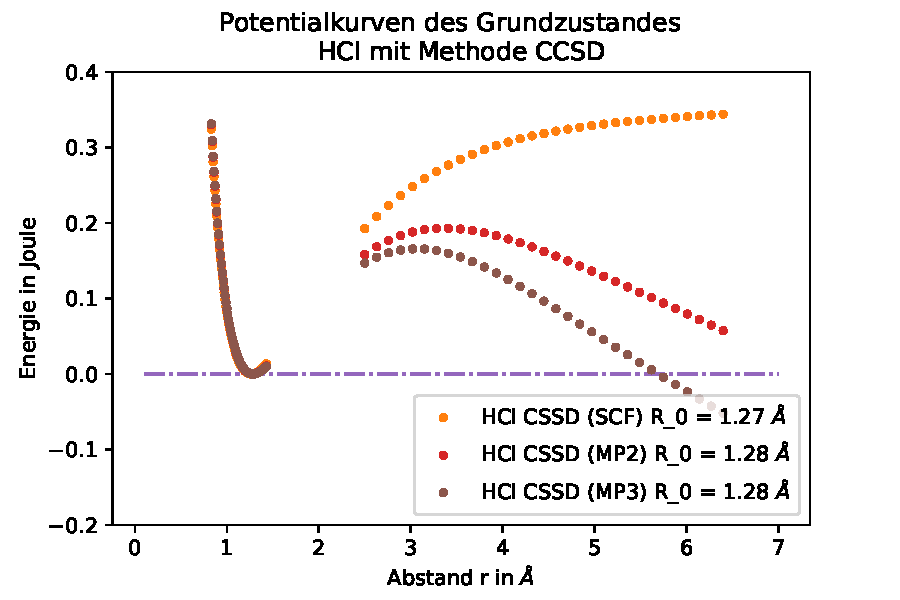
\includegraphics[width=\textwidth]{Bilder/HCl_CCSD}
\end{minipage}
\begin{minipage}{0.5\textwidth}
	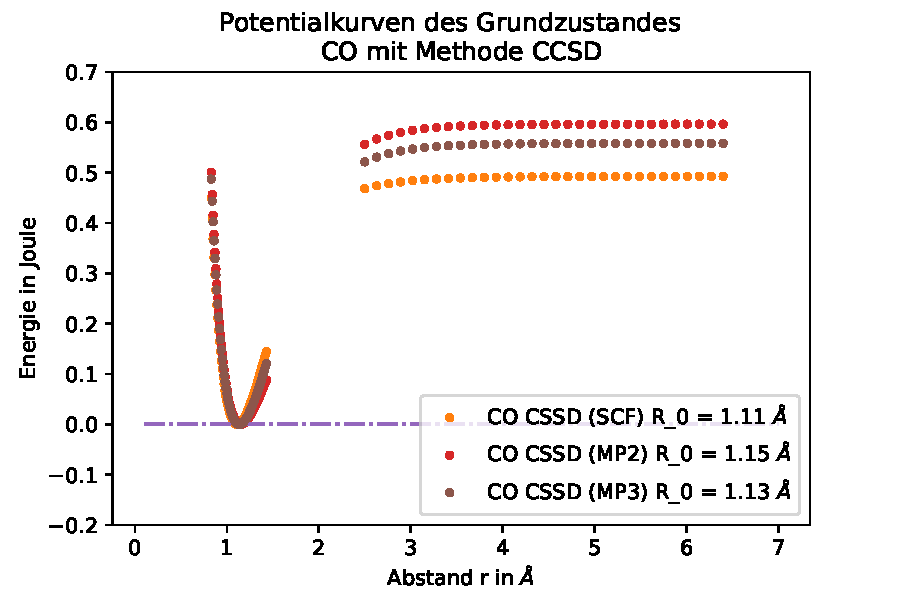
\includegraphics[width=\textwidth]{Bilder/CO_CCSD}
\end{minipage}
\caption{Das ist eine Caption}
	\label{HCl_CCSD}
\end{figure}


Der Verlauf der Werte, welche durch die CCSD Methode für CO, sowie HCl erhalten wurden, sind in Abbildung \ref{HCl_CCSD} aufgetragen worden. Bei der Betrachtung der Werte kann beobachtet werden, dass die Entwicklung durch Gaussian um das Minimum noch etwas genauer, als es mittels B3LYP der Fall war, gelungen ist. Jedoch beschreibt die Energie  nach der Dissoziation des Moleküle besonders bei HCl einen Verlauf der gänzlich den Erwartungen widerspricht. Die Kurven sollten eigentlich gegen einen Energiewert konvergieren. Dies erklärt , dass die mit diesem Datensatz zu findenden Dissoziationsenergien stark von den Literaturwerten abweichen.










%\end{document}
